%%%%%%%%%%%%%%%%%%%%%%%%%%%%%%%%%%%%%%%%%%%%%%%%%%%%%%%%%%%%%%%%%%%%%%%%%%%%%%%%%%%%
% Document data
%%%%%%%%%%%%%%%%%%%%%%%%%%%%%%%%%%%%%%%%%%%%%%%%%%%%%%%%%%%%%%%%%%%%%%%%%%%%%%%%%%%%
\documentclass[12pt]{article} %report allows for chapters
%%%%%%%%%%%%%%%%%%%%%%%%%%%%%%%%%%%%%%%%%%%%%%%%%%%%%%%%%%%%%%%%%%%%%%%%%%%%%%%%%%%%
\usepackage{preamble}
\newcommand{\vecx}{\boldsymbol{\vec{x}}}
\newcommand{\vecy}{\boldsymbol{\vec{y}}}

\begin{document}

\begin{center}
   \textsc{\large MATH 271, Homework 11}\\
   \textsc{Due December 7$^\textrm{th}$}
\end{center}
\vspace{.5cm}

\begin{problem}
Groups appear naturally as symmetries of physical systems. Each one of these symmetries manifests a \emph{conserved quantity} of the system. This is the extremely famous \emph{Noether's theorem}. For example, consider the harmonic oscillator equation
\[\
mx'' + k x = 0.
\]
We note that this equation is a second order, linear, homogeneous, and, most importantly, autonomous equation. 
\begin{enumerate}[(a)]
    \item Noting that the force $F=ma=mx''$, argue that the force itself is independent of time $t$.
    \item Write down the general solution to this equation.
    \item Show that energy is conserved for any general solution. That is, show
    \[
    E = \frac{1}{2}mx'^2 + \frac{1}{2}kx^2,
    \]
    is constant in time.
\end{enumerate}
\end{problem}

\begin{problem}
    Recall the hermitian inner product for vectors $\vecu,\vecv \in \C^n$ given by
    \[
    \langle \vecu,\vecv \rangle = \sum_{j=1}^n u_j v_j^*.
    \]
    For certain linear transformations $U \colon \C^n \to \C^n$ we have that the inner product is invariant under this transformation, i.e.,
    \[
    \langle U \vecu,U \vecv \rangle = \langle \vecu,\vecv \rangle.
    \]
    We refer to transformations of this kind as \emph{unitary}.
    \begin{enumerate}[(a)]
        \item Let $n=1$. Argue that all unitary transformations are of the form $e^{i\theta}$ for $\theta \in \R$. Elements of this form reside in the \emph{unitary group} $\operatorname{U}(1)$.
        \item For a transformation $U\colon \C^n \to \C^n$ show that we must have $UU^\dagger = I$, where $I$ is the identity transformation.
        \item Show that the set of unitary transformations form a group.
    \end{enumerate}
\end{problem}

\begin{problem}
When two groups $G_1$ and $G_2$ behave exactly the same as one another we say these groups are \emph{isomorphic}. That is,
\begin{enumerate}[i.]
    \item If the groups have a correspondence between each element. (E.g., For every element $g_1 \in G_1$ there is a corresponding element in $g_2 \in G_2$ and vice-versa).
    \item The product of corresponding elements is the same. (E.g., If we have $g_1 h_1 \in G_1$ then we have the corresponding element is $g_2 h_2 \in G_2$).
\end{enumerate}
This can be said more succinctly as there is a one-to-one and onto function $\varphi \colon G_1 \to G_2$ such that $\varphi(g_1h_1) = \varphi(g_1)\varphi(h_1)$.

In the previous problem we showed that an element of $\operatorname{U}(1)$ takes the form $e^{i\theta}$. A matrix in the group of rotation matrices in $\R^2$ (i.e., $\mathrm{SO}(2)$) can be written as
\[
\Rot_\theta = \begin{pmatrix} \cos \theta & - \sin \theta \\ \sin \theta & \cos \theta \end{pmatrix},
\]
for any choice of $\theta$. Argue that $\operatorname{U}(1)$ and $\operatorname{SO}(2)$ are isomorphic.  \emph{Hint: Go back to previous homeworks to see how we can faithfully represent complex numbers using matrices. This will give you a way to see that these groups behave analogously.}
\end{problem}

\begin{problem}
Another way to think about $\mathrm{SO}(2)$ is to consider it as the rotational symmetry group of the unit circle in the real plane $\R^2$.

Next, consider a cyclohexane $C_6H_{12}$ molecule:
    \begin{figure}[H]
        \centering
        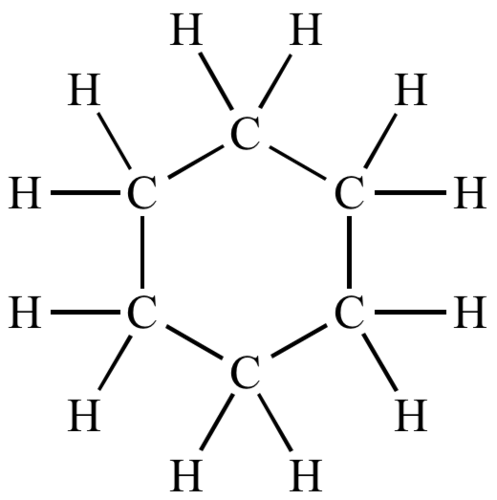
\includegraphics[width=.3\textwidth]{cyclohexane-500x500.png}
    \end{figure}
    \noindent This molecule also has rotational symmetry, but it is a smaller symmetry group than $\mathrm{SO}(2)$. We want to determine this rotational symmetry \emph{subgroup}.
\begin{enumerate}[(a)]
    \item This molecule looks much like a hexagon. Determine the external angles of a hexagon.
    \item Note that if we rotate a hexagon (or cyclohexane) by an external angle, then this leaves the molecule invariant (i.e., it looks no different). Using the external angle you found, write the rotation matrix for that angle and name this matrix $[g]$.
    \item We can \emph{generate} this group $C_6$ from $[g]$ by repeatedly multiplying $[g]$ with itself.  Show that there are only six elements in this group $C_6$.
    \item These are not all the symmetries of cyclohexane! Explain another symmetry operation that we could use that isn't captured by the rotations above.
\end{enumerate}
If you're interested, look up the group $D_{12}$ which is the \emph{dihedral group of order 12}. Or, taking it further, look at \url{https://en.wikipedia.org/wiki/Cyclohexane_conformation}
\end{problem}

\end{document}